\chapter{Result Analysis and Conclusion }\label{chap5}


\vspace*{40 ex}
%============================================================

\paragraph*{Outline:} This chapter presents the following:
\begin{enumerate}
	\setlength{\itemsep}{-0.3em}
	\item Result Analysis
	\item Conclusion
	\item The Future
	\item Hardware Requirement
\end{enumerate}
%============================================================

\newpage

\section{Result Analysis}
Regarding precision, the results were promising. We showed how a system trained on general image data can be used to detect rice crop insects and weed in a specific task (object detection), thus demonstrating the adaptability of the methods. In some cases, Faster R-CNN detected more insects or weed than the annotators of the original data had marked. These were labelled as false positives, despite clearly having the right species class by visual inspection.

On the other hand, the system did also make some actual normal mistakes. We deduced that this was most likely due to a lack of negative training examples. Further, we demonstrated the importance of postprocessing the results. Non-maximum suppression has a significant impact on the average precision. In general, overlapping objects and bounding boxes cause problems for object detection systems. We also showed that choice of the region generation method affects both speed and accuracy of the object detection system.

The results from the Google search images are shown in following figure 5.1 table.

\begin{figure}
	\subfloat{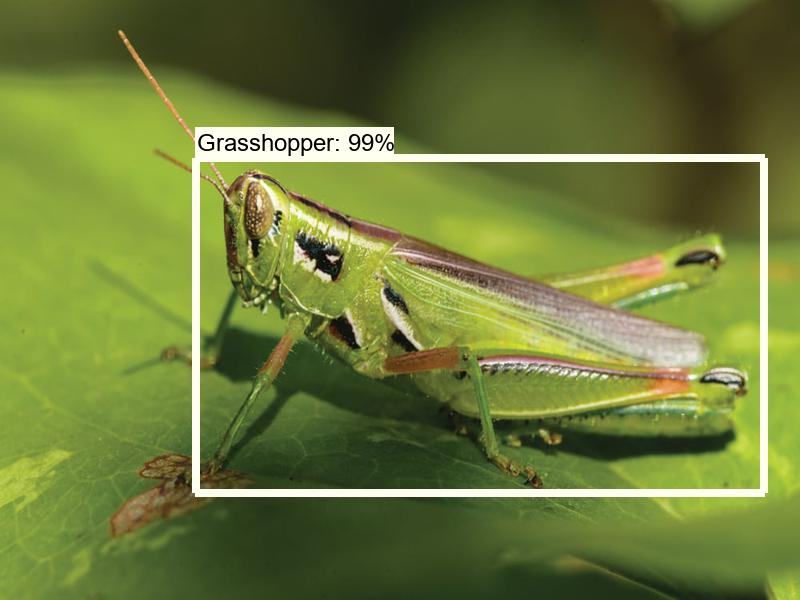
\includegraphics[width = 2in]{182}} 
	\subfloat{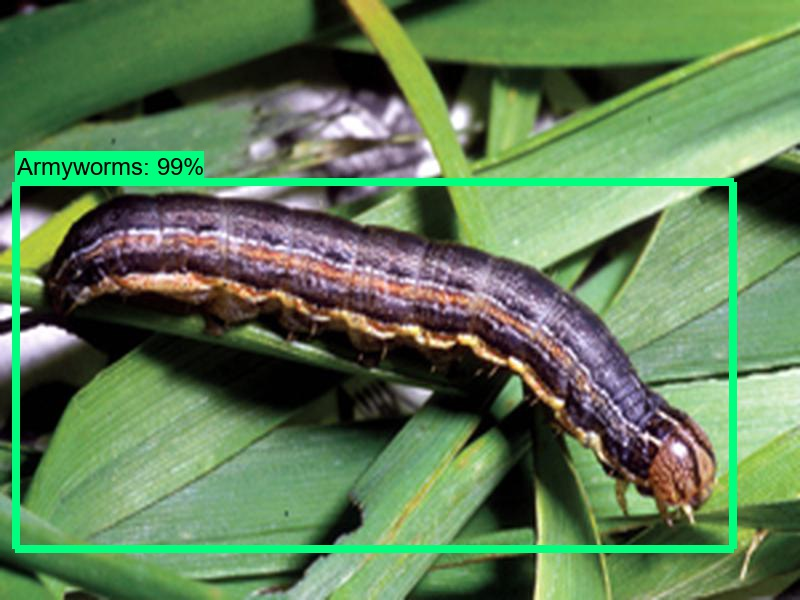
\includegraphics[width = 2in]{65}}
	\subfloat{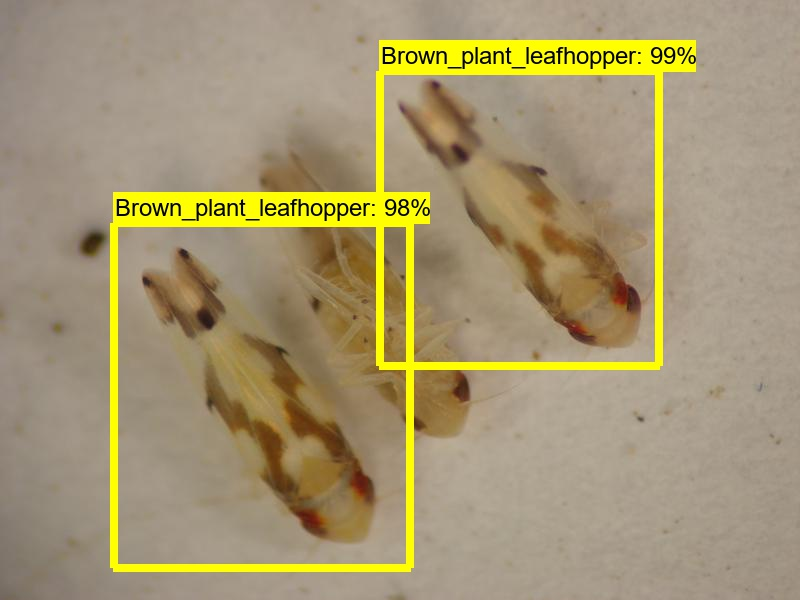
\includegraphics[width = 2in]{81}}\\
	\subfloat{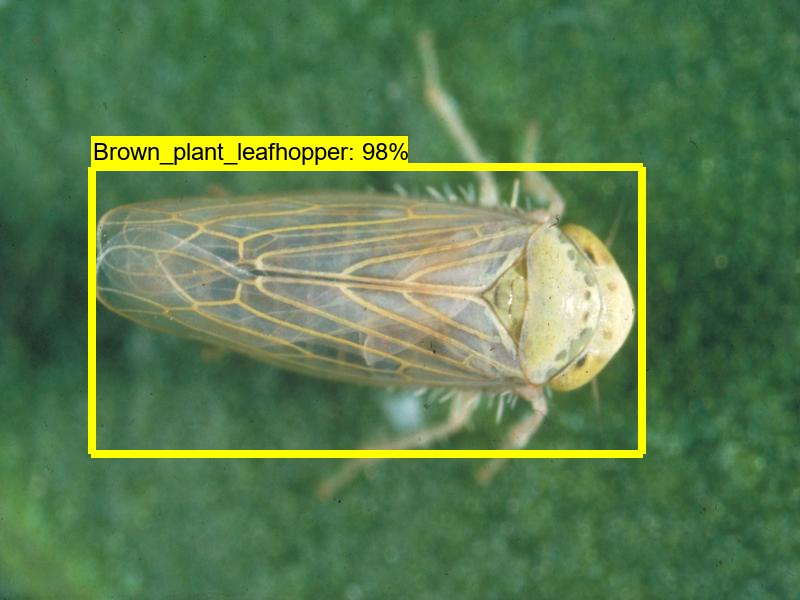
\includegraphics[width = 2in]{82}} 
	\subfloat{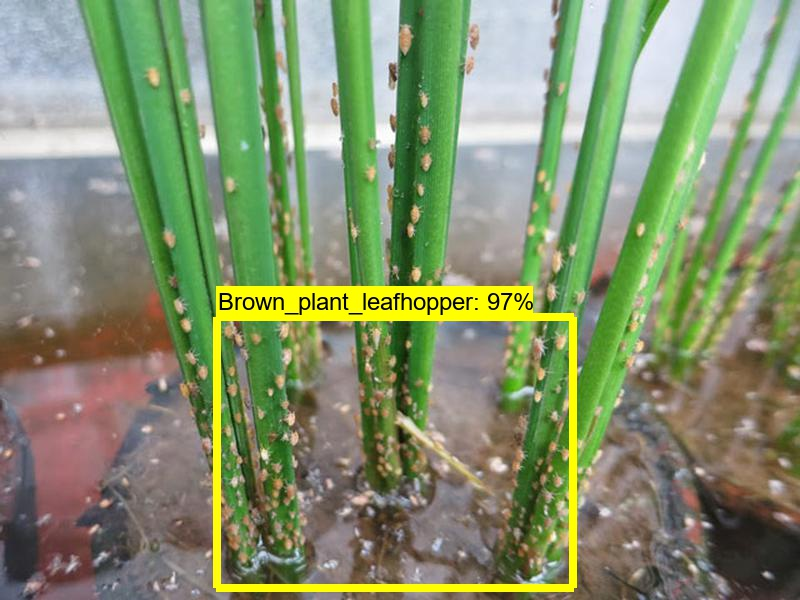
\includegraphics[width = 2in]{92}} 
	\subfloat{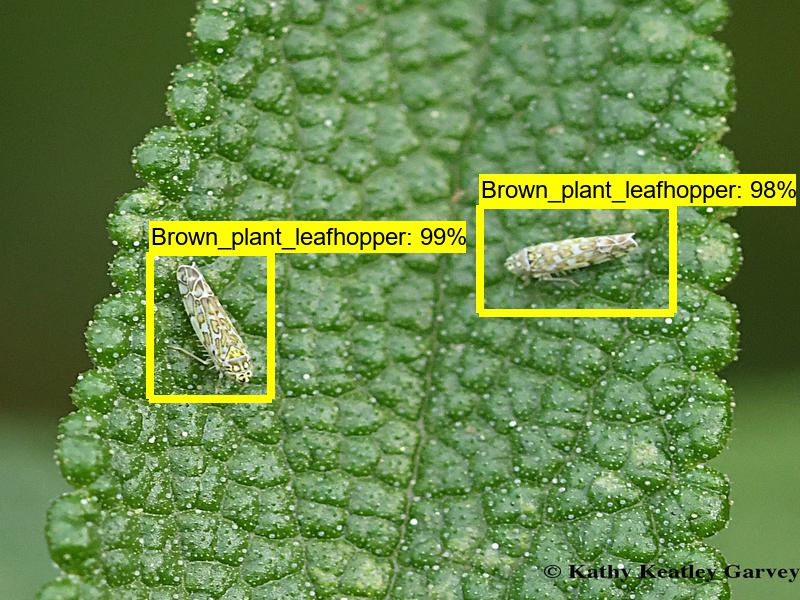
\includegraphics[width = 2in]{93}}\\
	\subfloat{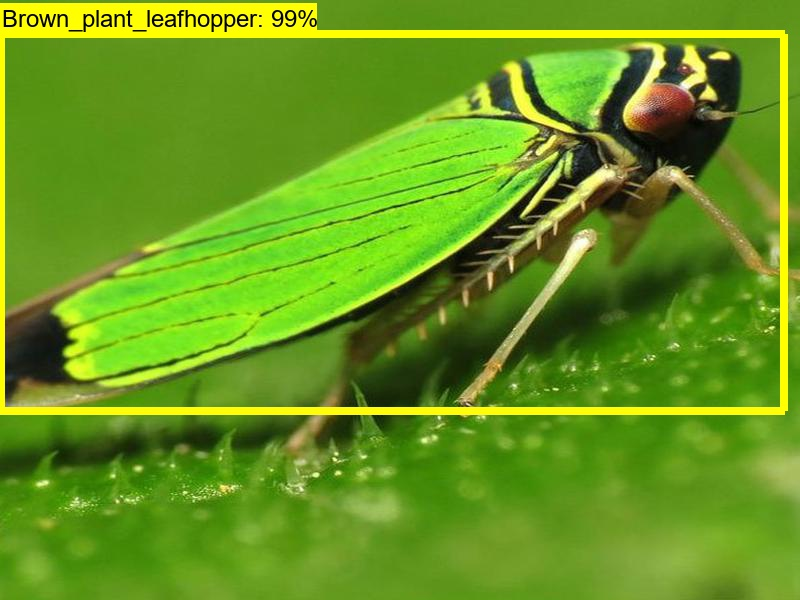
\includegraphics[width = 2in]{101}}
	\subfloat{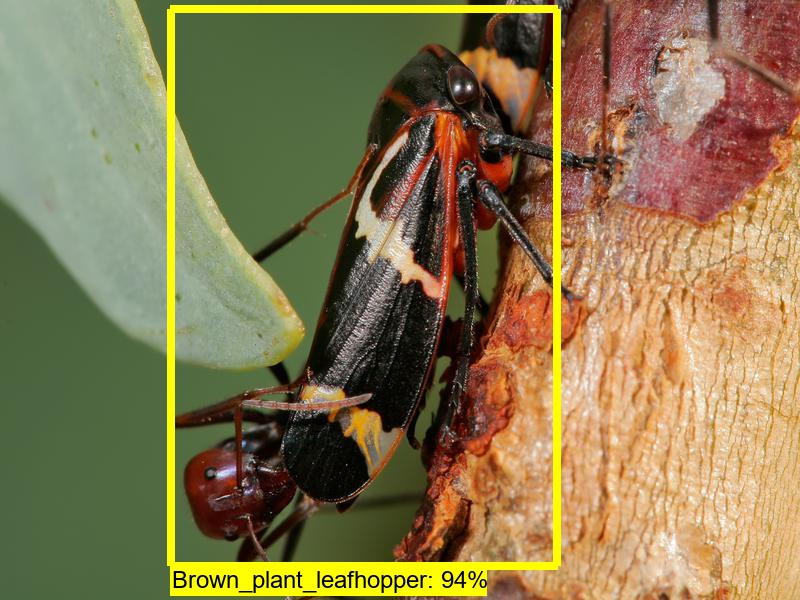
\includegraphics[width = 2in]{104}}
	\subfloat{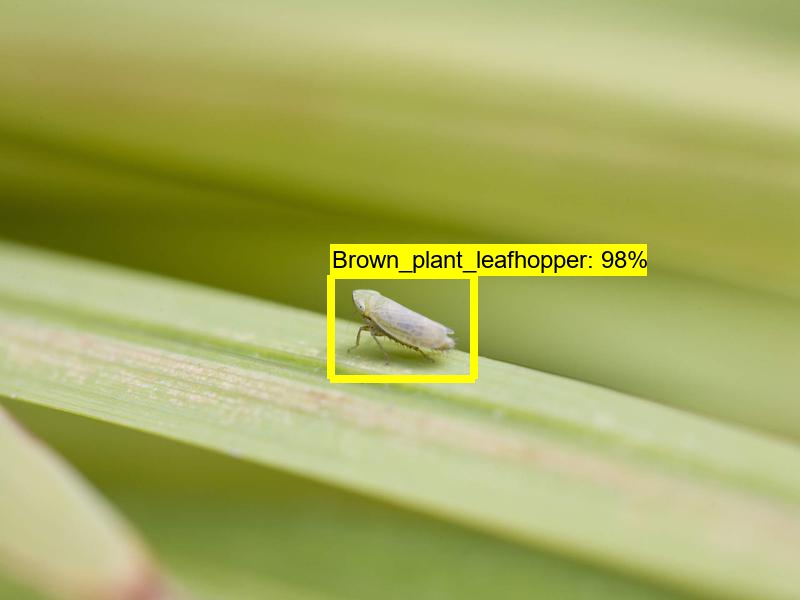
\includegraphics[width = 2in]{142}} \\
	\subfloat{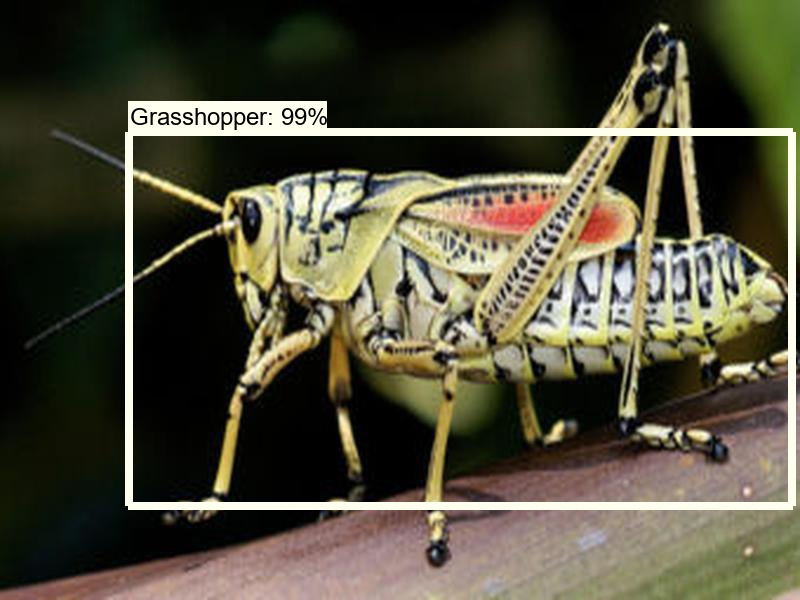
\includegraphics[width = 2in]{193}}
	\subfloat{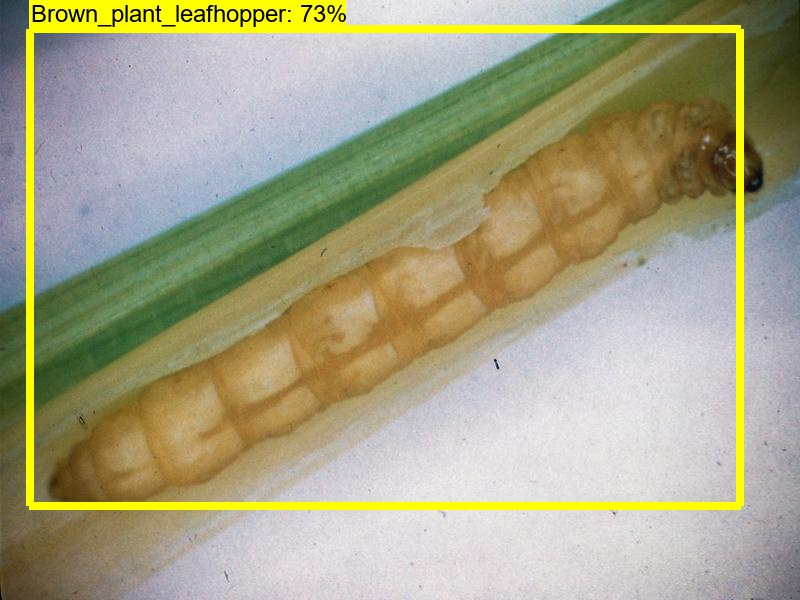
\includegraphics[width = 2in]{600}}
	\subfloat{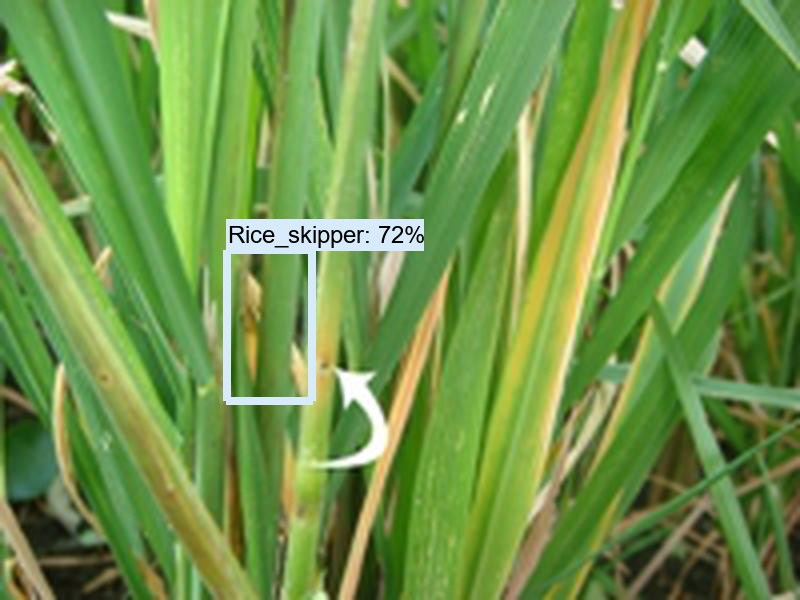
\includegraphics[width = 2in]{607}} \\
	\subfloat{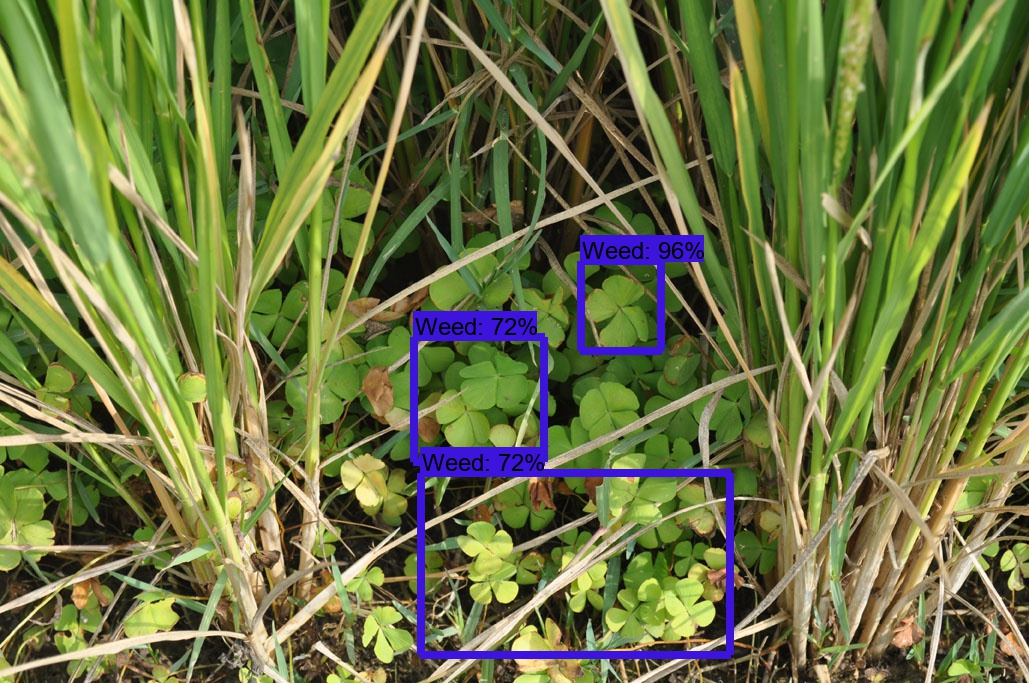
\includegraphics[width = 2in]{down25r}}
	\subfloat{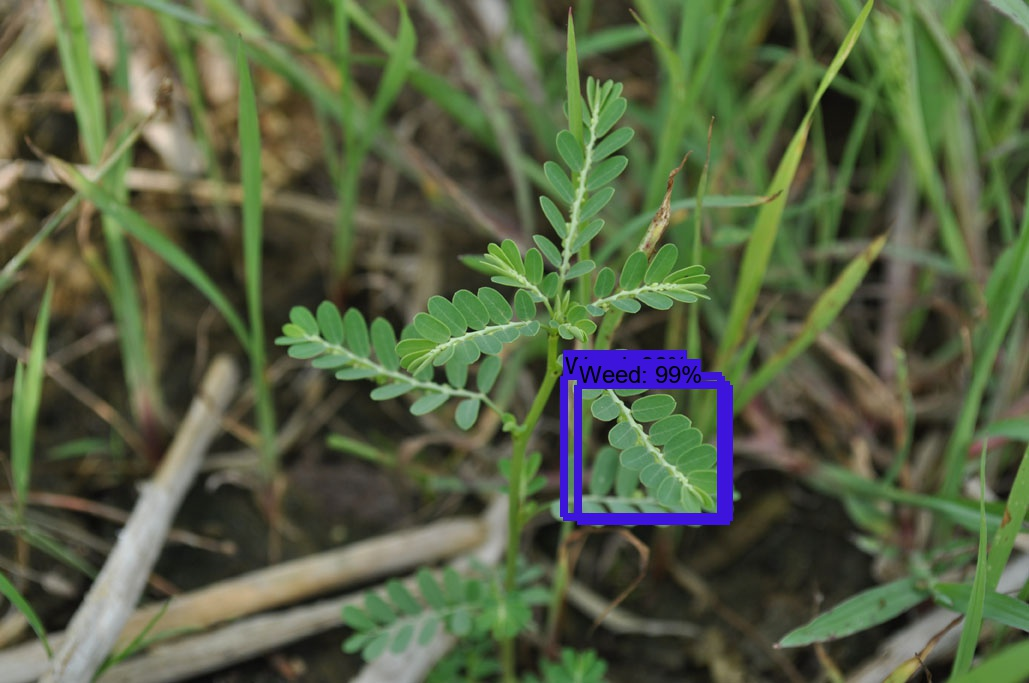
\includegraphics[width = 2in]{down26}}
	\subfloat{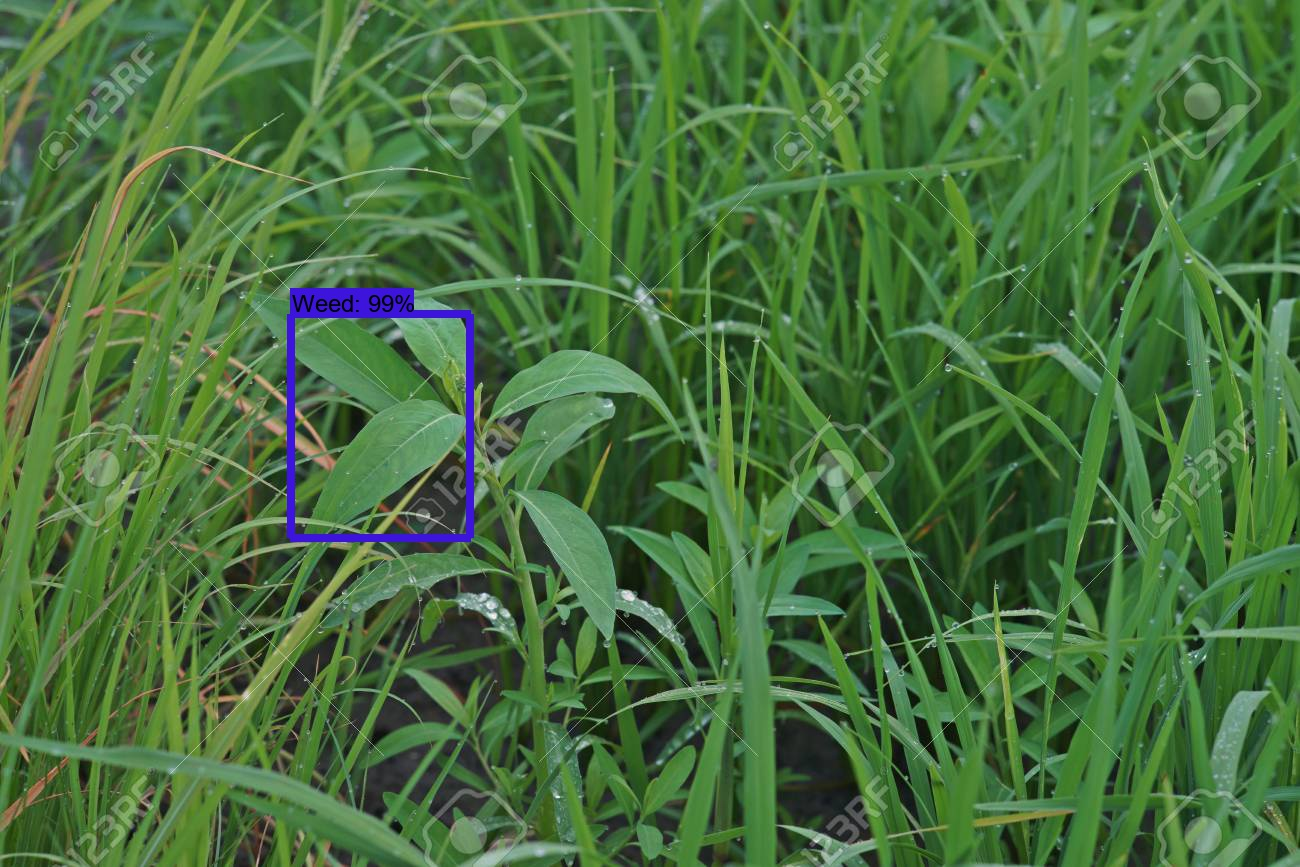
\includegraphics[width = 2in]{down2r}} \\
	
	\caption{Classification and Detection Result-I}
	\label{classification}
\end{figure}

\begin{figure}
	\subfloat{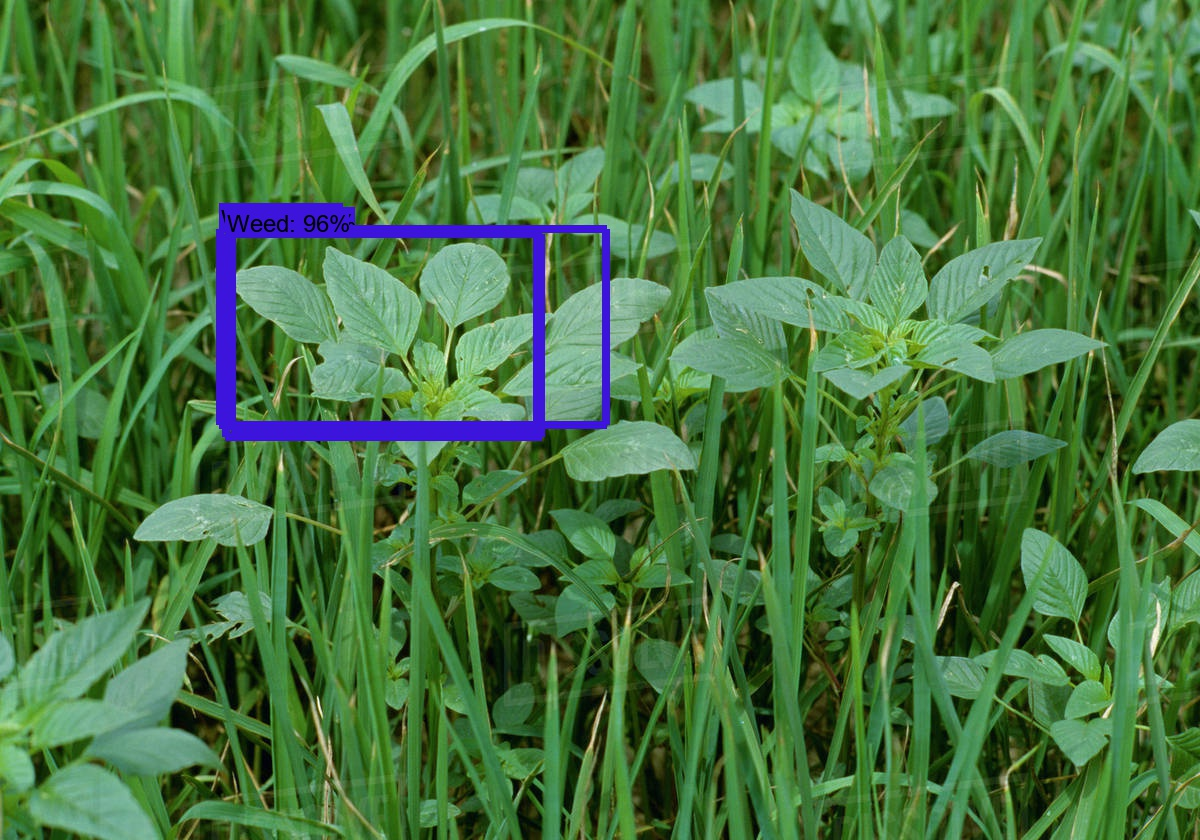
\includegraphics[width = 2in]{down17r}} 
	\subfloat{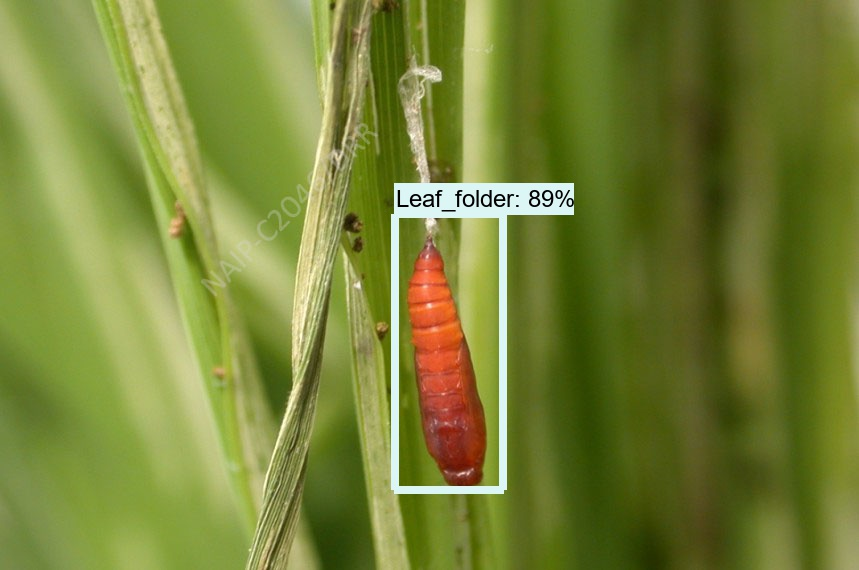
\includegraphics[width = 2in]{down7}}
	\subfloat{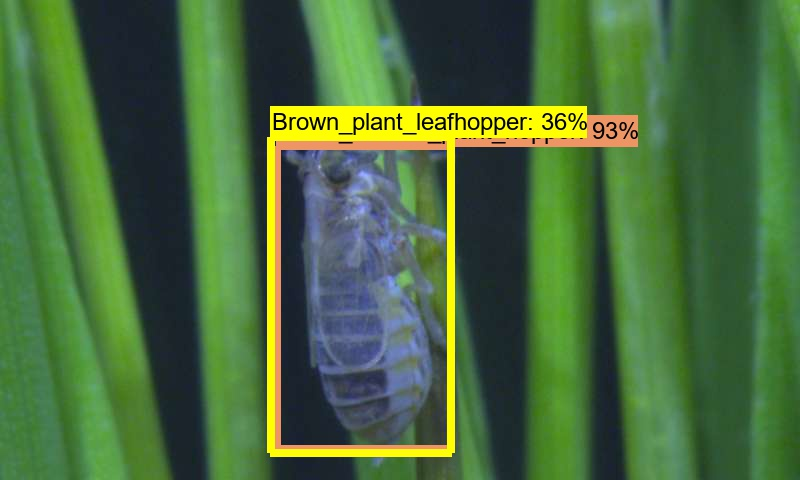
\includegraphics[width = 2in]{down1r}}\\
	\subfloat{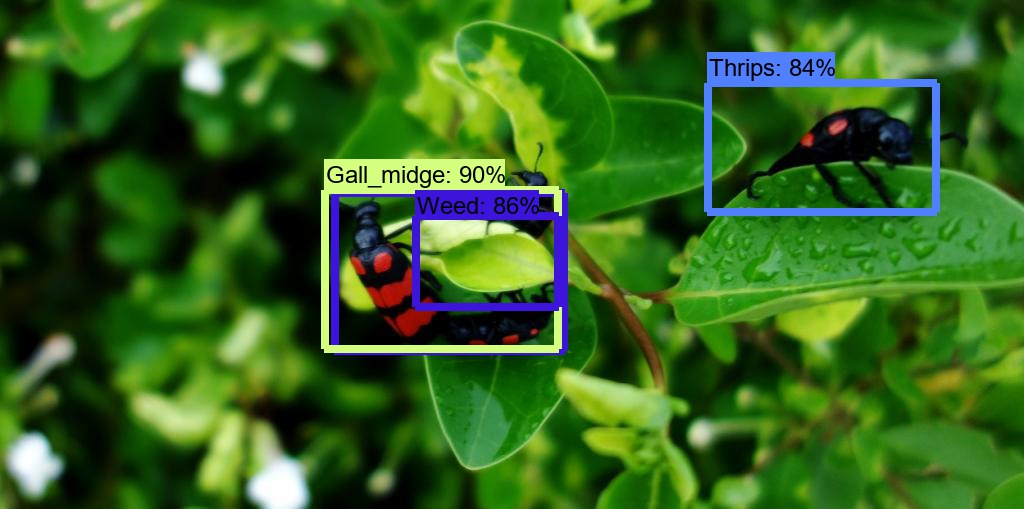
\includegraphics[width = 2in]{down6}} 
	\subfloat{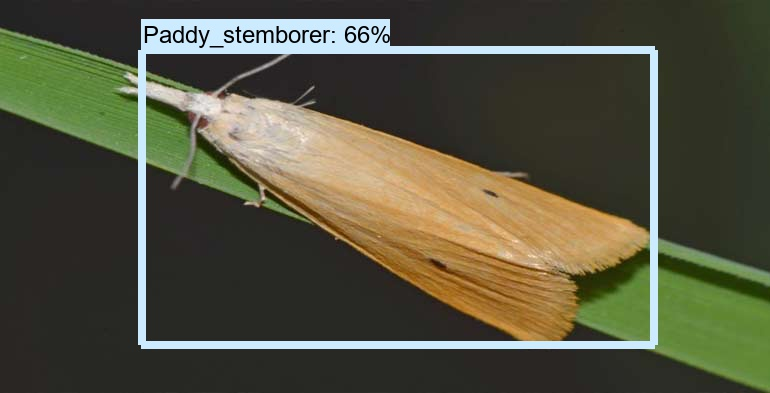
\includegraphics[width = 2in]{1_3}} 
	\subfloat{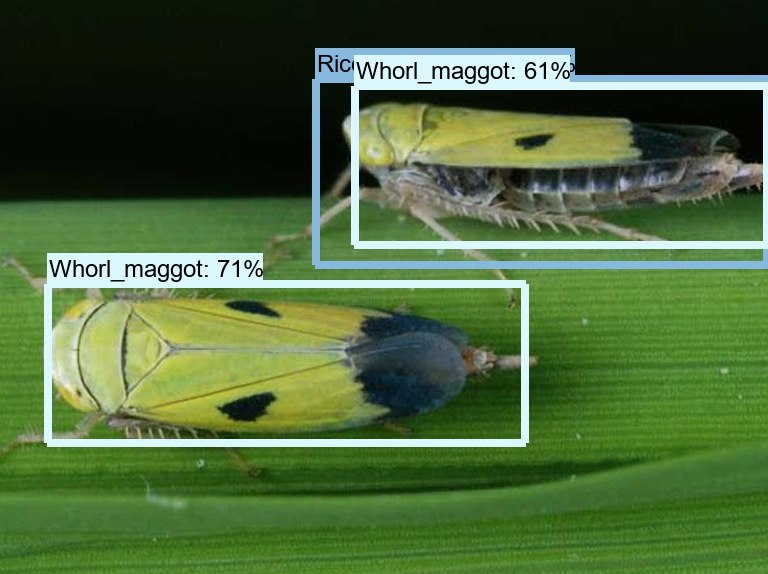
\includegraphics[width = 2in]{2}}\\
	\subfloat{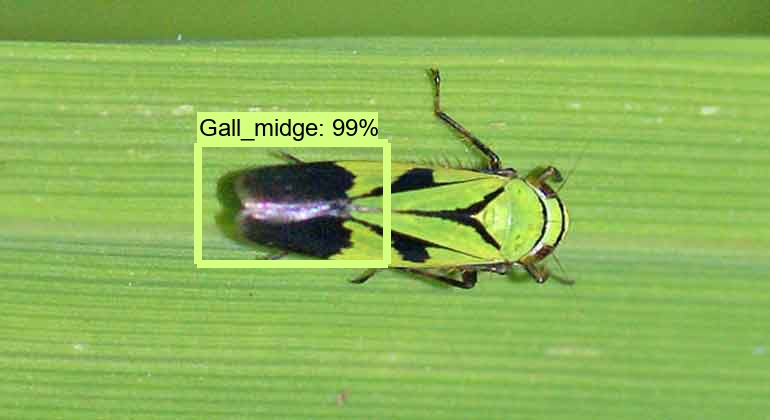
\includegraphics[width = 2in]{2_1}}
	\subfloat{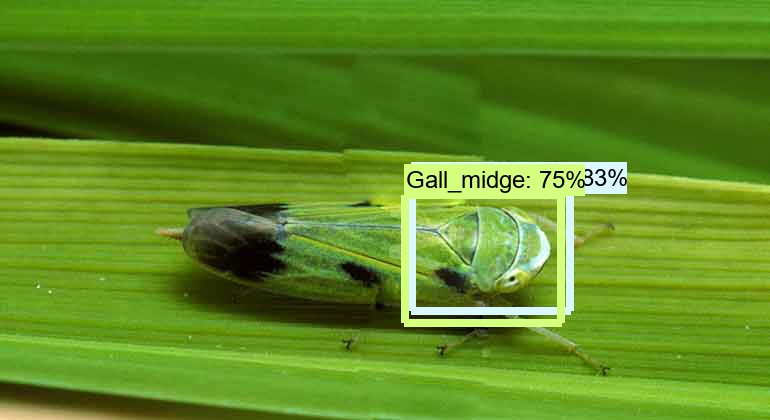
\includegraphics[width = 2in]{2_4}}
	\subfloat{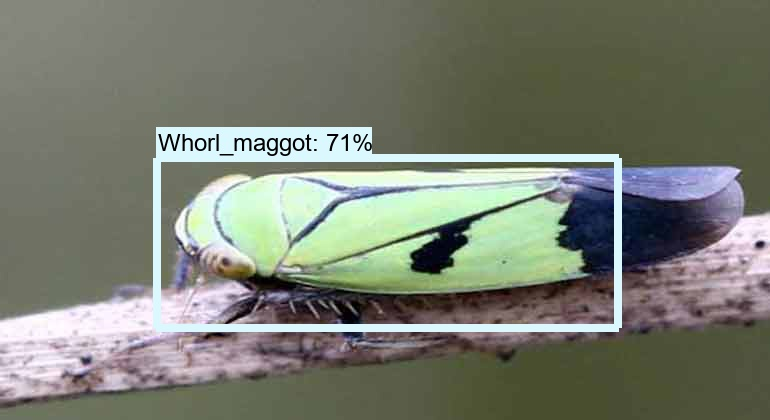
\includegraphics[width = 2in]{2_2}} \\
	\subfloat{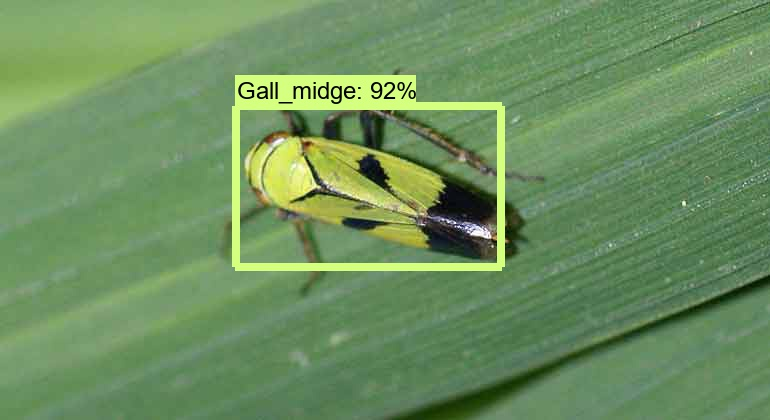
\includegraphics[width = 2in]{2_3}}
	\subfloat{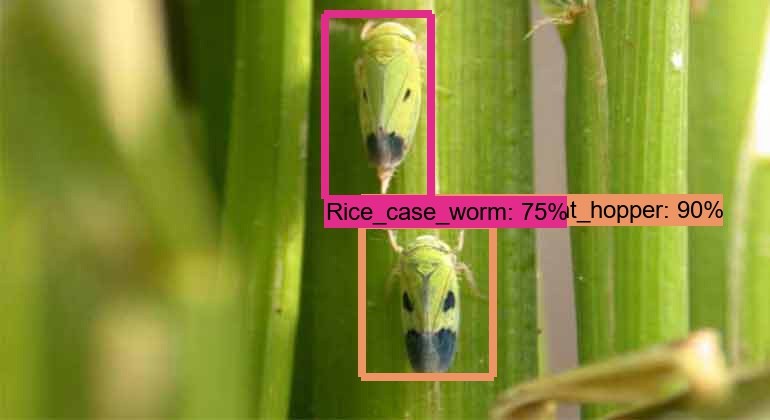
\includegraphics[width = 2in]{2_6}}
	\subfloat{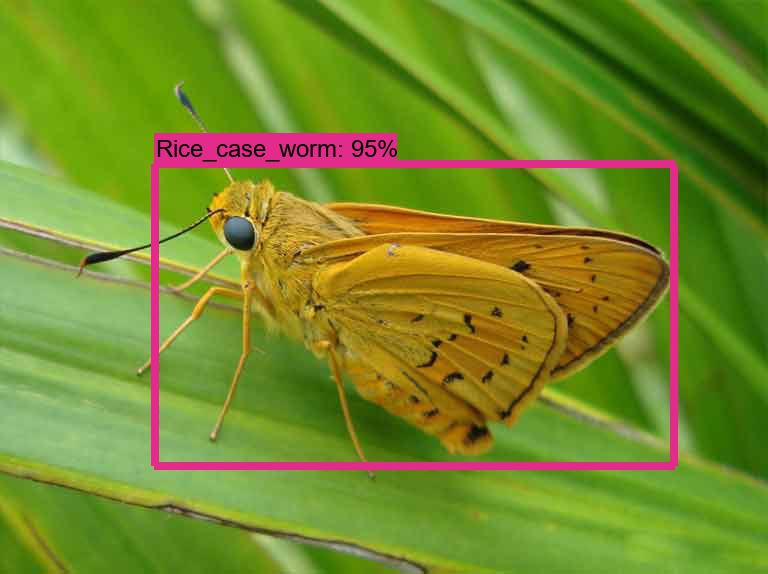
\includegraphics[width = 2in]{7}} \\
	\subfloat{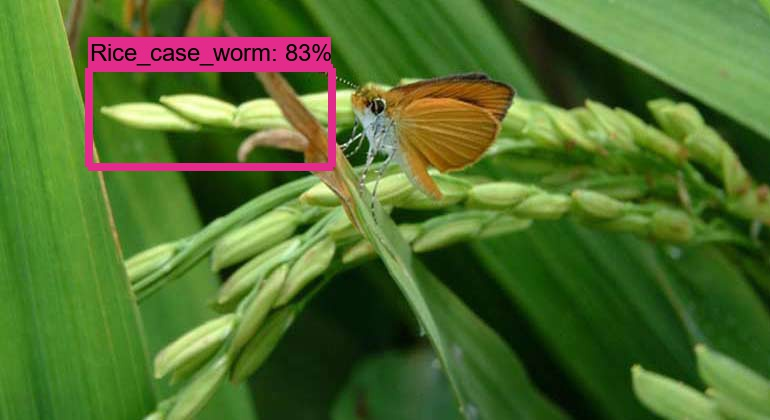
\includegraphics[width = 2in]{7_2}}
	\subfloat{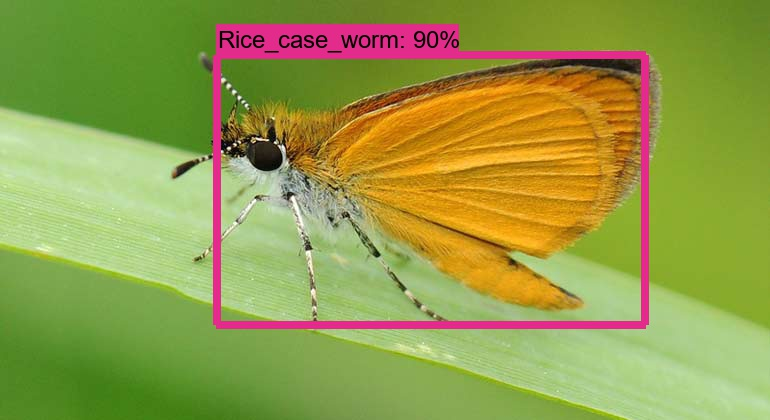
\includegraphics[width = 2in]{7_3}}
	\subfloat{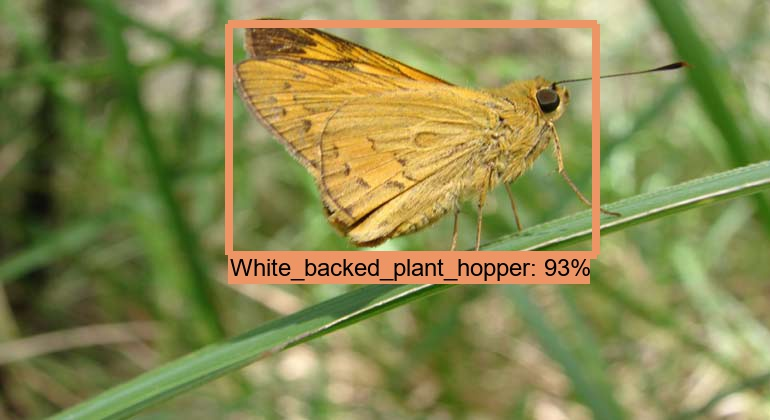
\includegraphics[width = 2in]{7_6}} \\
	
	\caption{Classification and Detection Result-II}
	\label{detection}
\end{figure}


\section{Conclusion}
An accurate and efficient object detection system has been developed which achieves comparable metrics with the existing state-of-the-art system. This project uses recent techniques in the field of computer vision and deep learning. Custom dataset was created using labelImg and the evaluation was consistent. This can be used in real-time applications which require object detection for pre-processing in their pipeline.

An important scope would be to train the system on a video sequence for usage in coltivation applications. Addition of a temporally consistent network would enable smooth detection and more optimal than per-frame detection.

\subsection{Overview}

We began the thesis with a review of the theoretical background. We explained how neural networks function and what object detection entails. We demonstrated why regular neural networks are insufficient to image-related tasks and how translation invariant convolutional networks provide an effective solution to many computer vision problems. 

Next, we demonstrated how convolutional object detection has evolved from the relatively slow R-CNN to the current optimized methods. This development is mostly not related to the structure of the convolutional network itself. Rather, it is related to how the convolutional network is used and to computation that takes place before and after the convolutional network. In the previous methods, there were many more separate phases involving preprocessing, region generation, computation of the fully connected layers and the final classification. In the latest methods, these phases have been increasingly integrated into the convolutional network itself, while keeping the basic CNN model intact. On the other hand, the 2016 winner of the ImageNet challenge is again a model composed of many separate components. Nonetheless, several computational bottlenecks have disappeared. Over the past few years, the speed of object detection has improved more dramatically than precision.

\subsection{Practice}
To experiment with a convolutional method in practice, we created a working PYTHON implementation of Faster R-CNN. We learned that the most challenging part of implementing a deep learning system is collecting the training data and performing the training itself. The publicly available datasets serve as a useful starting point for both research and practical implementations. Training time can be further shortened by using a pretrained network. Even if the final system does not feature the same objects classes as the benchmark data, visual problems are universal enough to benefit from detectors trained for a different problem. The optimal bottom-layers of a convolutional network are often similar regardless of the problem, just like human eye uses the same receptive fields for all visual tasks. Thus, it makes sense to initialize the layers using a pretrained network.

Related to the implementation, we also learned that there are no easy “out-of-the-box” solutions for effectively implementing convolutional networks. Current software tools, such as Caffe and MatConvNet, require specialist skills. If it is possible to use such tools, creating a working implementation is not too difficult. However, the tools are quite finicky regarding interoperability of software versions and hardware, especially if implementation is attempted on a GPU.


\section{The Future}

Exact study of the speed of the method variants was left outside the scope of the thesis. More detailed execution-time evaluation on consumer-level computers would be an interesting topic for further research. Many methods that claim “real time performance” can achieve this only on hardware costing thousands of euros. Even though hardware cost is not a major issue for certain applications such as self-driving cars and computer servers, which use expensive hardware in any case, more applications become practical after CNNs can be evaluated on home computers and mobile devices. Yet, our implementation showed that the methods have improved enough to detect objects in a few seconds on a consumer laptop, even though we did not measure this exactly.

One of the strengths of convolutional networks is their inherent translation invariance. Yet, taking the context of the whole image into consideration could potentially create an even more precise system. We experimented with a geometry-based inference system, which alters the probabilities of object detections based on their geometric plausibility. However, the method did not improve the accuracy of Faster R-CNN. We provided an analysis of how the geometric detection method functioned and determined that, while the method eliminated some false detections, it also created many new ones. The geometric method was also impractically slow. Yet, lessons learned from the study can be used to explore further ways of implementing context-sensitive object detection.

As explained in the previous chapter, a trend can be perceived in the literature of making detection systems wholly neural or convolutional. Just like a deep neural network learns to automatically learn the inherent features of an object class, an even deeper and more smartly used neural network could learn the probabilities of finding an object from a certain part of the scene. This would make a separate geometric inference method irrelevant. However, time will show if this is the route future research takes. As a Danish proverb says, it is difficult to make predictions, especially about the future.

\section{Hardware Requirement}
We have implemented and tested this thesis project with the help of  following hardware equipments :

\begin{enumerate}
	\setlength{\itemsep}{-0.3em}
	\item Windows 10 Operating System
	\item Intel i5-7200U 7th(Gen) CPU @ 2.50GHz- 2.71GHz
	\item CPU 8GB RAM
	\item NVIDIA Graphic 940MX with 4GB RAM
	\item NVIDIA Graphic Driver 430.86
	\item CUDA Toolkit 9.0
	\item cuDNN SDK v7.6.0
	\item Tensor-flow 1.13.1
\end{enumerate}

